\documentclass{article} % For LaTeX2e
\usepackage{iclr2026_conference,times}
\usepackage{amsmath,amssymb}
\usepackage{hyperref}
\usepackage{url}
\usepackage{booktabs}
\usepackage{graphicx}

\title{Simple Graph-Statistic Predictors of Random-Walk Cover Times\\on Small Connected Graphs}

\author{Anonymous Authors}

\newcommand{\cover}{C}

\begin{document}
\maketitle

\begin{abstract}
The expected cover time $\cover(G)$ of a simple random walk on a connected graph is classically bounded in terms of $n$ and $m$, e.g.\ $\cover(G)\le 2m(n-1)$. For small graphs these bounds are loose. We ask whether a predictor built from cheap statistics (vertices $n$, edges $m$, diameter $D$, maximum degree $\Delta$) can beat the general bound on graphs with $n\le 30$, and where it fails. On 236 synthetic connected graphs from 14 families, we estimate $\cover(G)$ by Monte Carlo with 2000 walks per graph (median relative standard error 1.2\%) and validate the estimator against exact linear-system values for 28 graphs with $n\le 8$. The general bound overestimates the cover time by a median factor of about $5.8$. A log-linear regression on $(n,m,D)$ reduces the median absolute relative error (APE) to 0.31 under 5-fold cross-validation, and adding $\Delta$ reduces it to 0.16; under leave-one-family-out evaluation the corresponding values are 0.37 and 0.23. Errors are small for paths, wheels, barbells, and trees and largest for grids, stars, and lollipops. The predictor is an empirical fit on a small synthetic sample, not a theorem.
\end{abstract}

\section{Introduction}
Cover time is the expected number of steps for a random walk to visit every vertex. Aleliunas et al.\ \citep{aleliunas1979} showed $\cover(G)\le 2m(n-1)$ for every connected graph, and Feige \citep{feige1995} sharpened worst-case bounds to order $n^3$ with a tight constant; Lovász's survey \citep{lovasz1993} gives the hitting-time machinery behind these results. These bounds are worst-case over graphs and start vertices, so for a specific small graph they can be off by a large factor. A practitioner who wants a rough number for a concrete graph with at most 30 vertices therefore has no good default.

We study a narrow, measurable question: for connected graphs with $n\le 30$, do a few statistics that are trivial to compute give a more accurate prediction than the general bound, and how does the error depend on graph type? We do not claim a new asymptotic result. Our contribution is (i) a Monte Carlo dataset of cover times with uncertainty estimates and exact validation on small graphs, (ii) a comparison of simple predictors under cross-validation and leave-one-family-out evaluation, and (iii) a description of the families on which the predictor is reliable and on which it fails.

\section{Method}
\paragraph{Target.} For a graph $G$ with $n$ vertices and $m$ edges, let $\cover(G)$ be the expected cover time with the start vertex drawn uniformly from $V$. Our Monte Carlo estimate is the mean of $R=2000$ independent walks; we report its standard error $s/\sqrt{R}$.

\paragraph{Features.} $n$, $m$, diameter $D$, and maximum degree $\Delta$. These are the only inputs to the predictors.

\paragraph{Predictors.} We compare: (a) the general bound $2m(n-1)$ with no fitting; (b) one-parameter scaling laws $\kappa\, nm$, $\kappa\, mD$, and $\kappa\, nmD$, with $\kappa$ fitted as the median of $\log(\cover/\text{stat})$; and (c) log-linear least squares $\log\cover = \beta_0+\beta_1\log n+\beta_2\log m+\beta_3\log D$, and the same with $+\beta_4\log\Delta$. The log-linear form is chosen because cover times span more than three orders of magnitude over the sample.

\paragraph{Evaluation.} Errors are absolute relative errors $|\hat\cover-\cover|/\cover$ computed out-of-fold. We use (i) 5-fold cross-validation repeated 20 times, and (ii) leave-one-family-out (LOFO), which tests transfer to an unseen graph family. Per-graph errors are the median over repetitions, and we report the median across graphs with a 95\% bootstrap CI (2000 resamples).

\section{Experimental setup}
\paragraph{Graphs.} All graphs are generated programmatically (no external data) by \texttt{code/cover.py}: paths, cycles, stars, wheels, complete graphs ($n\le 20$), grids, complete bipartite graphs, lollipops, barbells, random trees, random 3- and 4-regular graphs, Erd\H{o}s--R\'enyi graphs $G(n,p)$ conditioned on connectivity, and $Q_3$, $Q_4$, and the Petersen graph. The sample has $n\in[4,30]$ and 236 graphs in 14 families. Random families use seed 0.

\paragraph{Validation.} For 28 graphs with $n\le 8$ we compute $\cover(G)$ exactly by solving the linear system over states $(v,S)$ (current vertex, visited set). The maximum relative deviation of the Monte Carlo mean from the exact value is 2.5\%, and all deviations lie within three standard errors.

\paragraph{Reproduction.} \texttt{python3 code/cover.py --walks 2000 --seed 0 --out results/graphs.csv} then \texttt{python3 code/analyze.py --csv results/graphs.csv --out results/}. Numpy is the only dependency; the full run takes a few minutes on one CPU core.

\section{Results}
\begin{table}[t]
\centering
\caption{Median per-graph APE (lower is better) with 95\% bootstrap CIs over 236 graphs.}
\label{tab:main}
\begin{tabular}{lccc}
\toprule
Predictor & 5-fold CV & LOFO & 90th pct (CV)\\
\midrule
Bound $2m(n-1)$ (no fit) & 4.79 [3.91, 5.61] & 4.79 [3.96, 5.66] & 23.1\\
$\kappa\, nm$ & 0.59 [0.54, 0.66] & 0.63 [0.59, 0.71] & 3.16\\
$\kappa\, mD$ & 0.36 [0.30, 0.44] & 0.39 [0.33, 0.48] & 0.91\\
$\kappa\, nmD$ & 0.49 [0.41, 0.56] & 0.52 [0.43, 0.57] & 1.65\\
Log-linear $(n,m,D)$ & 0.31 [0.24, 0.38] & 0.37 [0.29, 0.46] & 0.74\\
Log-linear $(n,m,D,\Delta)$ & \textbf{0.16} [0.15, 0.18] & \textbf{0.23} [0.21, 0.26] & 0.46\\
\bottomrule
\end{tabular}
\end{table}

\paragraph{The general bound is loose here.} The ratio $\cover/(2m(n-1))$ has median $0.173$ and range $[0.007, 0.593]$, so $2m(n-1)$ overestimates the cover time by a median factor of about 5.8. The gap is largest on dense graphs: for $G(30,0.7)$ the ratio is $0.007$ (about $140\times$ over-estimation), and for $K_{20}$ it is $0.009$. The ratio is largest on paths ($\approx 0.59$), where the bound is nearly tight. Table~\ref{tab:main} shows that every fitted predictor beats the bound by an order of magnitude in median APE.

\paragraph{Feature choice matters.} Adding the maximum degree to $(n,m,D)$ roughly halves the error under both evaluation schemes. The one-parameter scalings are clearly worse than the log-linear fit, and $\kappa\, mD$ is the best of them. Fitted exponents for the log-linear $(n,m,D,\Delta)$ model are $\beta_1=0.51$, $\beta_2=0.11$, $\beta_3=1.33$, $\beta_4=0.82$ (full data), so the fit is not reducible to a single product law.

\paragraph{Where the predictor fails.} Figure~\ref{fig:pred} and the per-family table generated in \texttt{results/summary.md} show that error depends strongly on graph type. Under LOFO with $(n,m,D)$ the median APE is 0.05 on paths, 0.12 on wheels, 0.15 on barbells, and 0.21 on complete bipartite and tree graphs, but 0.70 on lollipops, 0.74 on 4-regular graphs, 0.80 on grids, and 0.68 on stars. Stars and lollipops have cover times dominated by a few high-degree or bottleneck vertices, which the four global statistics do not capture. Grids have a two-dimensional diffusive geometry that the diameter alone does not describe well.

\begin{figure}[t]
\centering
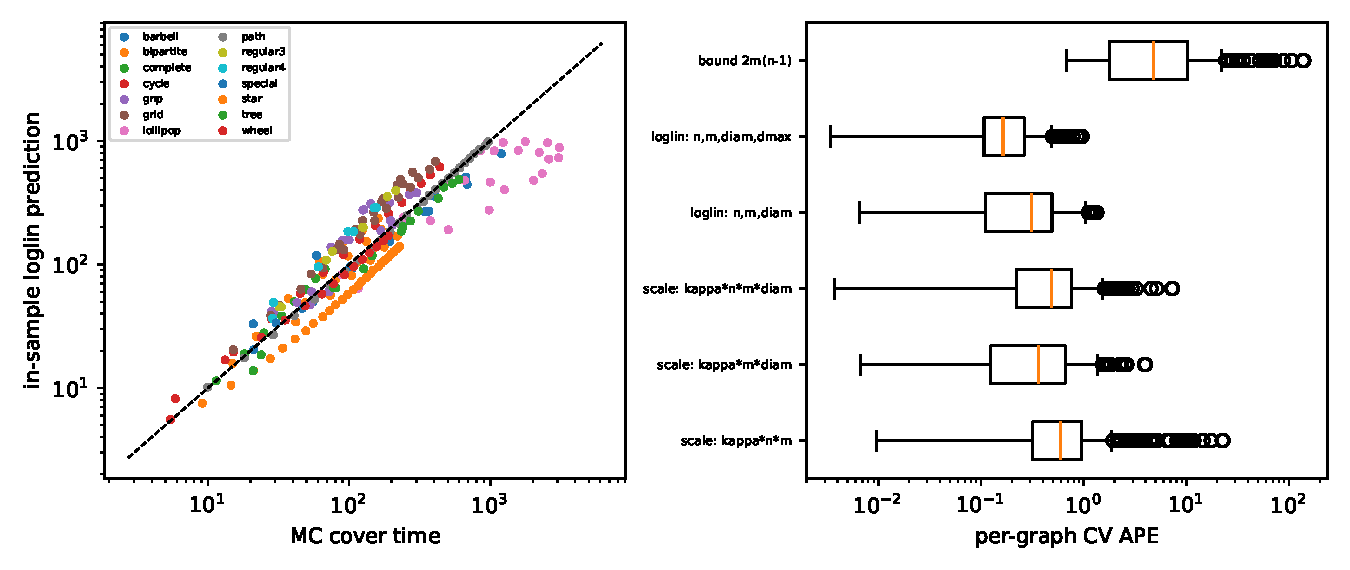
\includegraphics[width=\linewidth]{fig_predictions.pdf}
\caption{Left: in-sample log-linear $(n,m,D)$ prediction versus Monte Carlo cover time, colored by family (dashed: identity). Right: per-graph CV APE by predictor (log scale).}
\label{fig:pred}
\end{figure}

\section{Discussion and limitations}
The main finding is that a four-feature log-linear model gives cover-time estimates within about 16--23\% median error on this sample, against roughly 480\% for the general bound. This is a practical statement about small graphs from the families we tried, and it should not be read as a theorem or an asymptotic law. Limitations:
(1) The sample is synthetic, small (236 graphs), and uses a fixed set of families; the family composition drives the fitted coefficients, and LOFO errors are larger than CV errors for this reason.
(2) Cover times are averaged over a uniform start vertex; start-dependent cover time (for example from the leaf of a lollipop) is not predicted.
(3) We report uncertainty from Monte Carlo sampling and bootstrap over graphs, not over graph generators with different random seeds. Only one generator seed was run.
(4) Only four statistics were tested; we did not examine hitting-time-based or spectral features, which would be natural next candidates and might explain the grid and star failures.
(5) We did not check whether the predictor extrapolates beyond $n=30$.
Negative results are reported as observed: the one-parameter $\kappa\, nm$ law and the $\kappa\, nmD$ law are poor, and the grid and star families are not captured well by any predictor here.

\section{Conclusion}
On connected graphs with at most 30 vertices, simple graph statistics give predictions of the expected cover time that are far more accurate than the general bound $2m(n-1)$. Their accuracy is good on paths and tree-like or bipartite graphs and poor on grids, stars, and lollipops. Stronger features are needed for those families.

\bibliographystyle{iclr2026_conference}
\bibliography{refs}

\end{document}
